% Editable conceptual illustration. No plotted or measured data.
% Equal arrow lengths in panel (b) are schematic and set by construction.
\documentclass[tikz,border=5pt]{standalone}
\usepackage{times}
\usepackage{amsmath}
\usetikzlibrary{arrows.meta,calc}
\definecolor{ink}{HTML}{263241}
\definecolor{muted}{HTML}{637287}
\definecolor{refblue}{HTML}{2A78D6}
\definecolor{steerteal}{HTML}{1BAF7A}
\definecolor{planeedge}{HTML}{C6D5EB}
\definecolor{planefill}{HTML}{F5F8FD}
\definecolor{plateedge}{HTML}{91A7C4}
\definecolor{platefill}{HTML}{EFF4FB}
\begin{document}
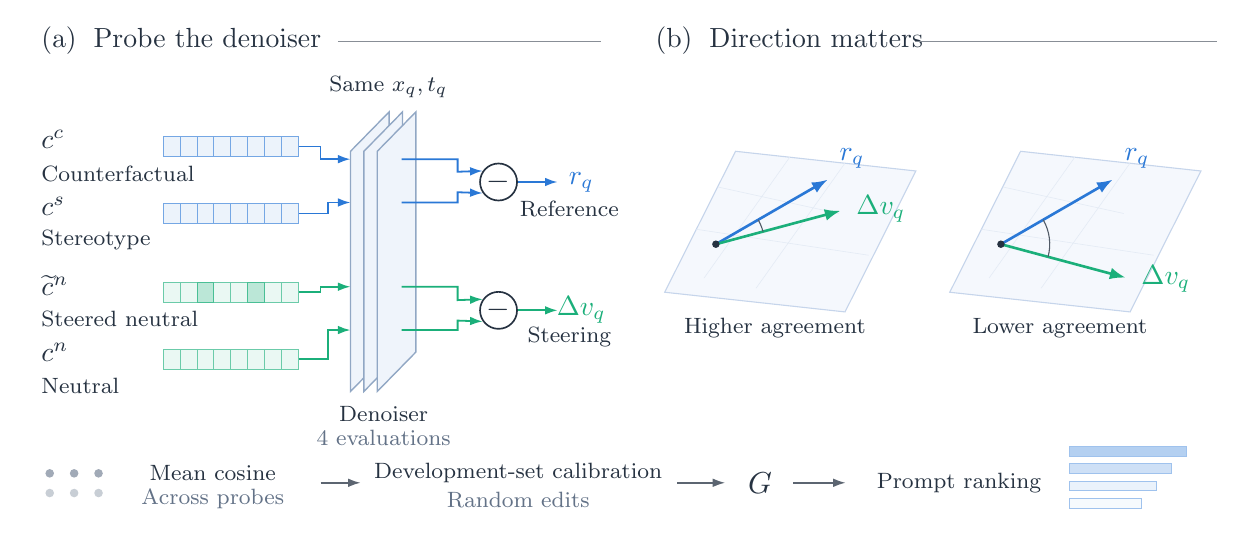
\begin{tikzpicture}[x=1cm,y=1cm,text=ink,
  font=\fontsize{8.5}{10}\selectfont,
  flow/.style={line width=.65pt,-{Latex[length=1.6mm,width=1.1mm]}},
  vector/.style={line width=.95pt,-{Latex[length=2mm,width=1.5mm]}},
  title/.style={font=\fontsize{10}{11}\selectfont,anchor=west},
  small/.style={font=\fontsize{8}{9}\selectfont},
  mathlabel/.style={font=\fontsize{10}{11}\selectfont}]
\path[use as bounding box] (-.05,-.12) rectangle (15.18,6.14);

% Restrained headers and a stable two-panel grid.
\node[title] at (0,5.97) {(a)\; Probe the denoiser};
\draw[ink!55,line width=.35pt] (3.89,5.97)--(7.23,5.97);
\node[title] at (7.80,5.97) {(b)\; Direction matters};
\draw[ink!55,line width=.35pt] (11.22,5.97)--(15.06,5.97);

% Four schematic embedding strips. These cell fills are not data.
\foreach \yy/\sym/\desc/\col in {
  4.63/{c^c}/Counterfactual/refblue,
  3.78/{c^s}/Stereotype/refblue,
  2.78/{\widetilde c^n}/{Steered neutral}/steerteal,
  1.93/{c^n}/Neutral/steerteal}{
  \node[anchor=west,mathlabel] at (0,\yy+.09) {$\sym$};
  \node[anchor=west,small] at (0,\yy-.34) {\desc};
  \foreach \k in {0,...,7}{
    \pgfmathsetmacro{\xx}{1.67+.215*\k}
    \draw[draw=\col!65,fill=\col!9,line width=.3pt]
      (\xx,\yy-.125) rectangle +(0.215,.25);
  }
}
\foreach \k in {2,5}{
  \pgfmathsetmacro{\xx}{1.67+.215*\k}
  \draw[draw=steerteal!80,fill=steerteal!30,line width=.3pt]
    (\xx,2.655) rectangle +(0.215,.25);
}

% A single shared module with four independent conditioned evaluations.
\node[small] at (4.53,5.39) {Same $x_q,t_q$};
\foreach \dx in {0,.17,.34}{
  \draw[draw=plateedge,fill=platefill,line width=.5pt]
    (4.05+\dx,1.52)--(4.54+\dx,2.02)--
    (4.54+\dx,5.07)--(4.05+\dx,4.57)--cycle;
}
\node at (4.47,1.24) {Denoiser};
\node[small,text=muted] at (4.47,.93) {4 evaluations};

% Inputs enter four different ports of the same denoiser.
\draw[flow,refblue] (3.39,4.63)--(3.67,4.63)--(3.67,4.47)--(4.05,4.47);
\draw[flow,refblue] (3.39,3.78)--(3.76,3.78)--(3.76,3.92)--(4.05,3.92);
\draw[flow,steerteal] (3.39,2.78)--(3.67,2.78)--(3.67,2.85)--(4.05,2.85);
\draw[flow,steerteal] (3.39,1.93)--(3.76,1.93)--(3.76,2.30)--(4.05,2.30);

% Ordered differences: first/upper output minus second/lower output.
\node[circle,draw=ink,line width=.6pt,fill=white,minimum size=4.7mm,
      inner sep=0pt,font=\fontsize{11}{11}\selectfont] (rsub) at (5.93,4.18) {$-$};
\node[circle,draw=ink,line width=.6pt,fill=white,minimum size=4.7mm,
      inner sep=0pt,font=\fontsize{11}{11}\selectfont] (dsub) at (5.93,2.55) {$-$};
\draw[flow,refblue] (4.70,4.47)--(5.41,4.47)--(5.41,4.31)--(rsub.145);
\draw[flow,refblue] (4.70,3.92)--(5.41,3.92)--(5.41,4.05)--(rsub.215);
\draw[flow,steerteal] (4.70,2.85)--(5.41,2.85)--(5.41,2.68)--(dsub.145);
\draw[flow,steerteal] (4.70,2.30)--(5.41,2.30)--(5.41,2.42)--(dsub.215);
\draw[flow,refblue] (rsub.east)--(6.68,4.18);
\draw[flow,steerteal] (dsub.east)--(6.68,2.55);
\node[mathlabel,text=refblue] at (6.98,4.18) {$r_q$};
\node[small] at (6.83,3.84) {Reference};
\node[mathlabel,text=steerteal] at (6.98,2.55) {$\Delta v_q$};
\node[small] at (6.83,2.21) {Steering};

% Two schematic response planes. Same reference and steering lengths.
\foreach \cx/\ang/\desc in {8.69/15/{Higher agreement},12.31/-15/{Lower agreement}}{
  \begin{scope}[shift={(\cx,3.39)}]
    \draw[draw=planeedge,fill=planefill,line width=.4pt]
      (-.65,-.61)--(.25,1.18)--(2.54,.93)--(1.64,-.86)--cycle;
    \begin{scope}
    \clip (-.65,-.61)--(.25,1.18)--(2.54,.93)--(1.64,-.86)--cycle;
    \draw[planeedge!48,line width=.22pt]
      (-.45,.22)--(1.94,-.14)
      (-.08,.75)--(1.56,.39)
      (-.15,-.43)--(.97,1.15)
      (.51,-.56)--(1.64,1.03);
    \end{scope}
    \draw[vector,refblue] (0,0)--(30:1.64);
    \draw[vector,steerteal] (0,0)--(\ang:1.64);
    \draw[ink!80,line width=.4pt] (\ang:.62)
      arc[start angle=\ang,end angle=30,radius=.62cm];
    \fill[ink] (0,0) circle[radius=1.35pt];
    \node[mathlabel,text=refblue,anchor=south west] at (30:1.67) {$r_q$};
    \node[mathlabel,text=steerteal,anchor=west] at (\ang:1.72) {$\Delta v_q$};
    \node at (.75,-1.06) {\desc};
  \end{scope}
}

% Quiet score-to-selection continuation: the full definition stays in the paper.
\foreach \xx in {.23,.54,.85}{
  \fill[muted!60] (\xx,.48) circle[radius=1.55pt];
  \fill[muted!35] (\xx,.23) circle[radius=1.55pt];
}
\node at (2.30,.49) {Mean cosine};
\node[small,text=muted] at (2.30,.15) {Across probes};
\draw[flow,ink!75] (3.67,.36)--(4.18,.36);
\node at (6.18,.49) {Development-set calibration};
\node[small,text=muted] at (6.18,.15) {Random edits};
\draw[flow,ink!75] (8.20,.36)--(8.81,.36);
\node[font=\fontsize{11}{11}\selectfont] at (9.25,.36) {$G$};
\draw[flow,ink!75] (9.67,.36)--(10.34,.36);
\node[anchor=west] at (10.61,.36) {Prompt ranking};
\foreach \yy/\ww/\shade in {.70/1.48/35,.48/1.29/23,.26/1.10/10,.04/.91/4}{
  \draw[draw=refblue!45,fill=refblue!\shade,line width=.3pt]
    (13.18,\yy) rectangle +(\ww,.12);
}
\end{tikzpicture}
\end{document}
